\documentclass[12pt,a4]{article}







\usepackage{graphicx,amsmath,amssymb,amsthm, boxedminipage,xcolor,amscd,amsbsy,latexsym,url,bm}

%\usepackage[lined,boxed]{algorithm2e}

\usepackage{algorithm}
\usepackage{algpseudocode}


\newtheorem{theorem}{Theorem}[section]
\newtheorem{proposition}[theorem]{Proposition}
\newtheorem{lemma}[theorem]{Lemma}
\newtheorem{corollary}[theorem]{Corollary}
\newtheorem{definition}[theorem]{Definition}

\newtheorem*{theorem*}{Theorem}
\newtheorem*{lemma*}{Lemma}
\newtheorem*{solution}{Solution}
\newtheorem*{proposition*}{Proposition}


\newtheorem{exercise}[theorem]{Exercise}
\newtheorem{exerciseD}[theorem]{*Exercise}
\newtheorem{exerciseDD}[theorem]{**Exercise}

\let\oldexercise\exercise
\renewcommand{\exercise}{\oldexercise\normalfont}

\let\oldexerciseD\exerciseD
\renewcommand{\exerciseD}{\oldexerciseD\normalfont}

%\let\oldexerciseD\exerciseD
%\renewcommand{\exerciseD}{\oldexerciseD\normalfont}

%\let\oldexerciseDD\exerciseDD
%\renewcommand{\exerciseDD}{\oldexerciseDD\normalfont}

\newcommand{\E}{\mathbb{E}}
%\newcommand{\nth}[1]{#1^{\textsuperscript{th}}}
\newcommand{\scalar}[2]{\ensuremath{\langle #1, #2\rangle}}
\newcommand{\floor}[1]{\left\lfloor #1 \right\rfloor}
\newcommand{\ceil}[1]{\left\lceil #1 \right\rceil}
\newcommand{\norm}[1]{\|#1\|}
\newcommand{\pfrac}[2]{\left(\frac{#1}{#2}\right)}
\newcommand{\nth}[1]{#1^{\textsuperscript{th}}}
\newcommand{\core}{\textnormal{core}}



\newif\ifsolution

\solutionfalse

\newcommand{\answer}[1]{
\ifsolution
{\color{blue} #1}
\else
\fi
}



\newcommand{\poly}{\textnormal{poly}}
\newcommand{\quasipol}{\textnormal{quasipol}}
\newcommand{\ssubexp}{\textnormal{stronglySubExp}}
\newcommand{\wsubexp}{\textnormal{weaklySubExp}}
\newcommand{\simplyexp}{\textnormal{E}}
\newcommand{\expo}{\textnormal{Exp}}



\newcommand{\N}{\mathbb{N}}
\newcommand{\nn}{\mathbb{N}_0^n}
\newcommand{\R}{\mathbb{R}}
\newcommand{\Z}{\mathbb{Z}}


\definecolor{darkgreen}{rgb}{0,0.6,0}

\date{}

\title{
\hbox{  Mathematical Foundations of Computer Science}
  \vspace{3mm}
{\normalsize CS 499,	Shanghai Jiaotong University,  Dominik Scheder\\
%\vspace{3mm}
Spring 2019}
}


\begin{document}

\maketitle

%\begin{quotation}
%  You are welcome to discuss the exercises in the discussion
%  forum. Please take them serious. Doing the exercises is as important
%  than watching the videos.
%
%  I intentionally included very challenging exercises and marked them
%  with one or two ``$*$''. No star means you should be able to solve
%  the exercises without big problems once you have understood
%  the material from the video lecture. One star means it requires 
%  significant additional thinking. Two stars means it is not 
%  unlikely that you will fail to solve them, even once you have understood
%  the material and thought a lot about the exercise. Don't feel bad
%  if you fail. Failure is part of learning.
%
%  This is the first time this course is online. Thus there might be mistakes
%  (typos or more serious conceptual mistakes) in the exercises. I will be 
%  grateful if you point them out to me!
%\end{quotation}



\newtheorem*{solution}{Solution}
\setcounter{section}{3}

\begin{center}
  \large\textbf{Group: navigator} 
\end{center}
\begin{center}
  \begin{tabular}{rl}
 Xu Huan  & 517021910724 \\
 Tianyao Shi     &     517021910623 \\
Chenxiao Yang    &    517021910540  \\
Jiaqi  Zeng      &     517021910882  \\
  \end{tabular}
\end{center}

\newpage




\section{Random Walks}


\subsection{Random Walks on $\{0,\dots, k\}$}

Consider a random walk starting at $j$. Let $p_j$ be the probability that this walk reaches $k$ before
it reaches $0$. I showed in the lecture that $p_j  = j/k$. Let me give you an alternative proof.
\begin{proof}
   For $t \in \N_0$ let $X_t$ denote the position after $t$ steps. So $X_0= j$, $X_1 \in \{j-1,j+1\}$, and so on.
   Note that if $X_t = l$ then $\E[X_{t+1}] = \frac{l-1}{2} + \frac{l+1}{2} = l$. This implies that in fact
   $\E[X_t] = j$ for all $t\in \N_0$. Thus, it must also hold for $t = T$, where $T$ is the time it 
   takes until the walk reaches $0$ or $k$. Therefore, $\E[X_T] = j$. 
   
   Now let's compute $\E[X_T]$ in a different way: by definition of $T$, we will be at $0$ or at $k$. 
   The latter happens with probability $p_j$, the former with probability $1-p_j$. Thus,
   \begin{align*}
      \E[X_T] = k \cdot p_j + 0 \cdot (1-p_j) \ .
   \end{align*}
   Therefore, $j = \E[X_T] = k \cdot p_j$ and $p_j = j /k$.
\end{proof}
\begin{exercise}
    Explain why this proof is wrong.
    \begin{solution}
    \begin{align*}
      \E[X_T] = k \cdot p_j + 0 \cdot (1-p_j) \ .
   \end{align*}
   This equation is wrong. $T$ is the time it takes until walk reaches $0$ or $k$, but it doesn't promise that it definitely reaches $0$ or $k$ after $T$ steps. Starting from $j$, There can be other terminal positions.
    \end{solution}
\end{exercise}
\subsection{Random Walks on $\Z$}

Consider the biased random walk on $\Z$. We start at some point $j \geq 1$. In every step,
we go one step left with probability $p$ and one step right with probability $1-p$. In the lecture we
have seen three things: (1) if $p < 1/2$ then with some positive probability, this walk never reaches $0$;
(2) if $p \geq 1/2$ then the walk reaches $1$ with probability $1$; (3) if $p=1/2$ then 
although the walk reaches $0$ with probability $1$, the expected number of steps until it does so is infinite.
Let $T$ denote the number of steps until we reach $0$ when the walk starts at $1$; if the walk never
reaches $0$, we define $T = \infty$.

\begin{exercise}
   Suppose $p > 1/2$. 
   \begin{enumerate}
   \item Show that $\E[T]$ is finite. That is, the sum $\sum_{n = 1}^\infty n \Pr[T = n]$ converges.
   \item Compute $\E[T]$. \textbf{Hint.} Recall that
   \begin{align*}
   \E[T] = \sum_{n = 0}^\infty (2n+1)  \, C_n \,  p^{n+1} \, (1-p)^n \ .
   \end{align*}
   Apply some tricks from the previous lectures to evaluate this sum.
   \end{enumerate}
\begin{solution}
	\begin{enumerate}
		\item We give the explicit form of $\E[T]$ as
		$$
		\E[T]=\sum_{n = 0}^\infty (2n+1)  \, C_n \,  p^{n+1} \, (1-p)^n,
		$$ 
		where we have $$C_n=\frac{{2n \choose n}}{n+1}=\frac{(2n)!}{(n+1)!\,n!}\leq 4^n.$$
		We can prove it by induction, but for short we shall leave it as what we already know. Besides, when $p>1/2$, we have $p(1-p)<1/4$. Now consider the infinite series $A$
		$$
		A=\sum_{n = 0}^\infty (2n+1)  \, 4^n \,  p^{n+1} \, (1-p)^n\geq \E[T],
		$$
		if it converges, then $\E[T]$ converges. We have
		$$\lim_{n\rightarrow \infty}\frac{a_{n+1}}{a_n}=\lim_{n\rightarrow \infty}\frac{2n+3}{2n+1}\cdot 4\cdot p(1-p)=4p(1-p)<1.
		$$
		So by the ratio test, the series converges when $p>1/2$. Therefore, $\E[T]$ also converges.
		\item We find the hint is somewhat misleading in this sub-problem, as it implies that we had better use calculus to solve this problem. However, it is simpler to compute $\E[T]$ if we consider it as what expectation is. Say, we are at 1 and go with one move. With probability $p$ we are at 0 and have no movement eversince, and with probability $1-p$ we are at 2 and need to first go back to 1, then go to 0. That is,
		$$
		\E[T]=1+p\cdot \E[0\rightsquigarrow0]+(1-p)\cdot(\E[2\rightsquigarrow1]+\E[T]).
		$$
		Note that to reach 1 from 2 is identical to to reach 0 from 1. Therfore $\E[2\rightsquigarrow1]=\E[T]$, and we can give
		$$\E[T]=1+2(1-p)\E[T].
		$$
		We solve it and get $\E[T]=\frac{1}{2p-1}$.
	\end{enumerate}
\end{solution}
\end{exercise}

\begin{exercise}
   Suppose $p < 1/2$. Let $T$ be the number of steps 
   until we reach $0$. On the one hand, we can compute $\E[T]$ as follows:
   \begin{align*}
     \E[T] &  = \sum_{n=0}^\infty (2n+1) C_n p^{n+1} (1-p)^n \\
     & = p \,  \sum_{n=0}^\infty (2n+1) C_n (p \, (1-p))^n \\
     & < \sum_{n=0}^\infty (2n+1) \, 4^n \, (p \, (1-p))^n  < \infty \ ,
   \end{align*}
   since $C_n \leq 4^n$ and $p \, (1-p) < 1/4$. On the other hand, $\E[T] = \infty$ for the unbiased
   random walk, so for the $p$-biased random walk with $p<1/2$, it should take even
   longer to reach $0$, right?    Explain what went wrong here.
\begin{solution}
	For one thing, the inequalities above mean anything but $\E[T] \neq \infty$. For another, there is some fixed positive probability that random walk goes infinite steps right and never goes left. Taking that case into consideration, $\E[T]$ is obviously $\infty$.
\end{solution}
\end{exercise}


If $p=1/2$ then $\E[T]$ is infinite. We have shown this already last week in two different ways.
However, what about $\E\left[\frac{1}{T}\right]$? This should exist. After all, 
\begin{align*}
     \sum_{n=1}^\infty \frac{1}{n} \Pr[T = n] \leq \sum_{n=1}^\infty \Pr[T=n] = 1 \ ,
\end{align*}
so the sum is bounded, each term is non-negative, and so the series must converge. I think
computing $\E\left[\frac{1}{T}\right]$ is quite nasty. So let me give you a simpler problem:                                                                              
\begin{exercise}
   Compute $\E\left[\frac{1}{T+1}\right]$.
	\begin{solution}
   		\begin{align*}
   		\E[\frac{1}{T+1}] & = \sum_{n=0}^\infty \frac{1}{2n+2} C_n p^{n+1} (1-p)^n \\
   		& = \frac{1}{2(1-p)}\sum_{n=0}^\infty \frac{1}{n+1} C_n (p(1-p))^{n+1} \\
   		& = \frac{1}{2(1-p)} \int_{0}^{x}  \sum_{n=0}^\infty C_n x^n \,dx \\
   		& = \frac{1}{2(1-p)} \int_{0}^{p(1-p)} \frac{1}{p}\sum_{n=0}^\infty C_n p^{n+1}(1-p)^n \, d(p(1-p)) \\
   		& = \frac{1}{2(1-p)} \int_{0}^{p(1-p)} \frac{1}{1-p} \, d(p(1-p)) \\
   		& = \frac{1}{2(1-p)} \int_{0}^{p(1-p)} \frac{1-2p}{1-p} \, dp \\
   		& = p + \frac{ln(1-p+p^2)}{2(1-p)}
   		\end{align*}
	\end{solution}
\end{exercise}


\subsection{Monster Wars and Robot Wars}

Alice and Bob are the captains of a team of monsters. Each monster has some strength $a > 0$. If two 
monsters of strengths $a$ and $b$ fight, the first monster wins with probability $\frac{a}{a+b}$ and the second
with probability $\frac{b}{a+b}$. The winning monster devours the loser and its strength increases to $a+b$.
The losing monster gets eaten (obviously) and dies.

Alice heads a team of $m$ monsters of strengths $a_1,\dots,a_m$. Bob's monsters have strengths
$b_1,\dots,b_n$. In each round, Alice and Bob each choose a monster to be sent into the arena. There,
the two monsters then fight, the winning monster devours the loser, and returns to its team (with increased strength). 
After at most $n+m-1$ rounds, one
team has died completely. The other team is declared winner.

\begin{exercise}
    Show that the probability of Alice's team winning does not depend on the order in which Alice and Bob
    send their monsters into the arena. 
    Compute the exact winning probability, it terms of $a_1,\dots,a_m, b_1,\dots, b_n$.
\end{exercise} 

\textbf{Solution.} Recall that in a random walking problem, $p_j=j/k$ (the probability that a random walk starting at $j$ and reaches $k$ before it reaches $0$). Therefore, we can treat monster competition as a random walking process.\par
To build a random walking model, we make following definitions:\\
\begin{center}
	\begin{tabular}{c|c}
		\hline
		\textbf{Notation} & \textbf{Definition}\\
		\hline
		\hline
		$A_t$& The set of each monster's strength in Alice's team after round t.\\
		\hline
		$B_t$& The set of each monster's strength in Bob's team after round t.\\
		\hline
		$p(X)$& The position of monster strength set X, i.e, $p(X)=\sum_{x_i\in X} x_i$\\
		\hline
	\end{tabular}
\end{center}\par 
The initial position of Alice's team is $p(A_0)=\sum_{i=1}^m{a_i}$, Bob's team is $p(B_0)=\sum_{i=1}^n{b_i}$. Also, a team is declared winner when the other team's position reaches $0$.\par 
Consider that after round $t$, the position of Alice's team is $p(A_t)$, the position of Bob's team is $p(B_t)$. Suppose monster $a_i$ and $b_j$ are fighting in round $t+1$:
	$$Pr\Big (p(A_{t+1})=p(A_t)+b_j\Big) = a_i/(a_i+b_j)$$
	$$Pr\Big(p(A_{t+1})=p(A_t)-a_i\Big) = b_j/(a_i+b_j)$$\par 
	\begin{figure}[htbp]
	    \centering
        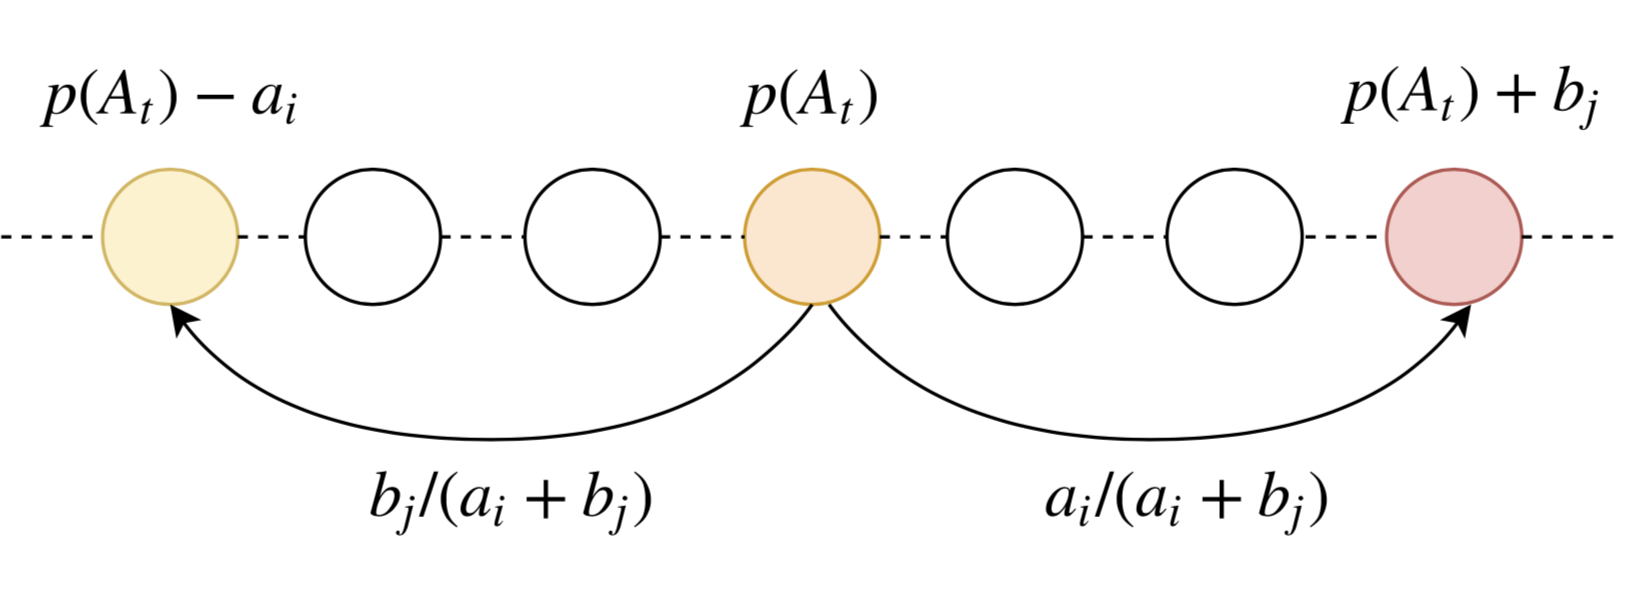
\includegraphics[width=0.8\textwidth]{Fig-transition.png}
        \caption{Position Transition from Round $t$ to Round $t+1$}
	\end{figure}
Recall that in a random walking process, let $p_j$ be the probability that a walk starts at $j$ and reaches $k$ before it reaches $0$, $p_j=j/k$ as showed in class.\par
Also, a fight between monsters with strength $a_i$ and $b_j$ can be treated as: $a_i$ monsters with strength $1$ are fighting with $b_i$ monsters of strength $1$ until there is no monster in one side (Without loss of generalization, we assume $a_i$ and $b_j$ are positive integers).\par
Therefore, we can treat the monster fighting as a random walk. Correspondingly, this walk model starts at $p(A_0)=\sum_{i=1}^m{a_i}$ and either end up at $p(A_{n+m-1})=0$ or $p(A_{n+m-1})=\sum_{i=1}^m{a_i}+\sum_{i=1}^n{b_i}$.\par 
According to the random walking formula, the probability of Alice's team winning the game is $\sum_{i=1}^m{a_i}/(\sum_{i=1}^m{a_i}+\sum_{i=1}^n{b_i})$, Bob's team winning the game is $\sum_{i=1}^n{b_i}/(\sum_{i=1}^m{a_i}+\sum_{i=1}^n{b_i})$.
%--------------------------END---------------------------

\quad\\\\\\\
Now let us repeat this setting with a slight change: it's not monsters but robots, and again strength-$a$-robot
beats strength-$b$-robot with probability $\frac{a}{a+b}$. The only difference: the losing robot explodes, and 
the strength of the winning robot does not change.

\begin{exerciseD}
    Show that the probability of Alice's team winning does not depend on the order in which Alice and Bob
    send their monsters into the arena.
    \textbf{Warning.} This is much more difficult. 
\end{exerciseD}

%---------------------------BEGIN---------------------------
\textbf{Solution.}\\ 
{\color{blue}Observation:} Every robot war with fixed robot order can be represented as a state-transition diagram. As shown in Figure \ref{ex461}, the state in $i^{th}$ row and $j^{th}$ column means ``robot $a_i$ fights with robot $b_j$".
	\begin{figure}[htbp]
	    \centering
        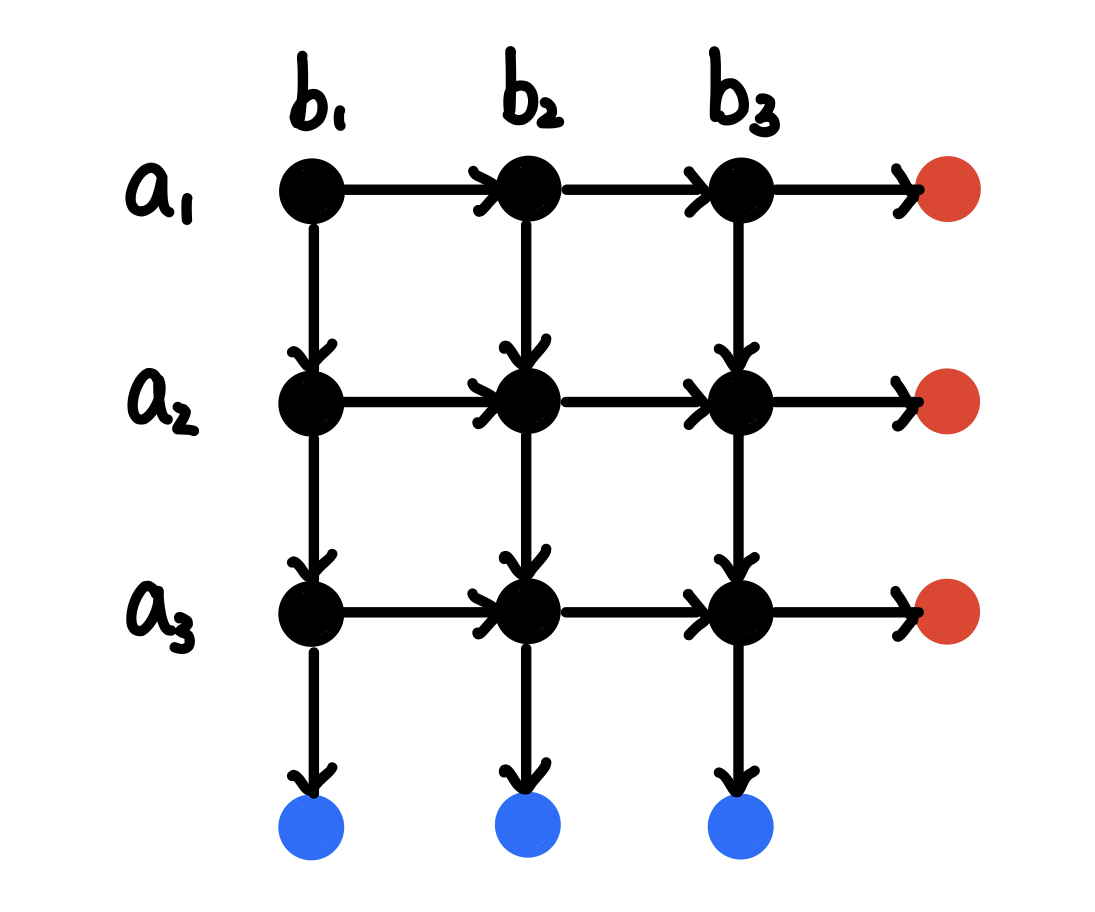
\includegraphics[width=0.4\textwidth]{Fig-stateDiagram.jpeg}
        \caption{An example of robot war state-transition diagram}
        \label{ex461}
	\end{figure}\\
We define  $P_{i,j}$ as the probability of this state occurring in the game. Correspondingly:
$$P_{i+1,j+1} = P_{i+1,j} \cdot  \frac{a_{i+1}} {a_{i+1}+b_j} + P_{i,j+1} \cdot  \frac{b_{j+1}} {a_{i}+b_{j+1}}$$
Suppose number of robots in team A is $m$, team B is $n$. Then:
$$\begin{cases} Pr(\text{team A win the game})=\sum_{i=1}^n P_{m+1,i} = \text{Sum(blue vertices in the figure)}\\
Pr(\text{team B win the game})=\sum_{i=1}^m P_{i,n+1} = \text{Sum(red vertices in the figure)} \end{cases}$$
{\color{blue}Lemma 1:} If there are only two robots in team A, the probability of A losing the game won't change after switching the order of those two robots.\\
Define $P_{ij}$ as the probability before switching, $P'_{ij}$ the probability after switching. A stronger proposition is that $P_{3,i} = P'_{3,i}$ for all $i\in{1,2,\cdots,n}$, \\\\
{\color{blue}Proof Lemma 1:}  The corresponding state-transition diagram is shown in Figure \ref{ex462}.\\
	\begin{figure}[htbp]
	    \centering
        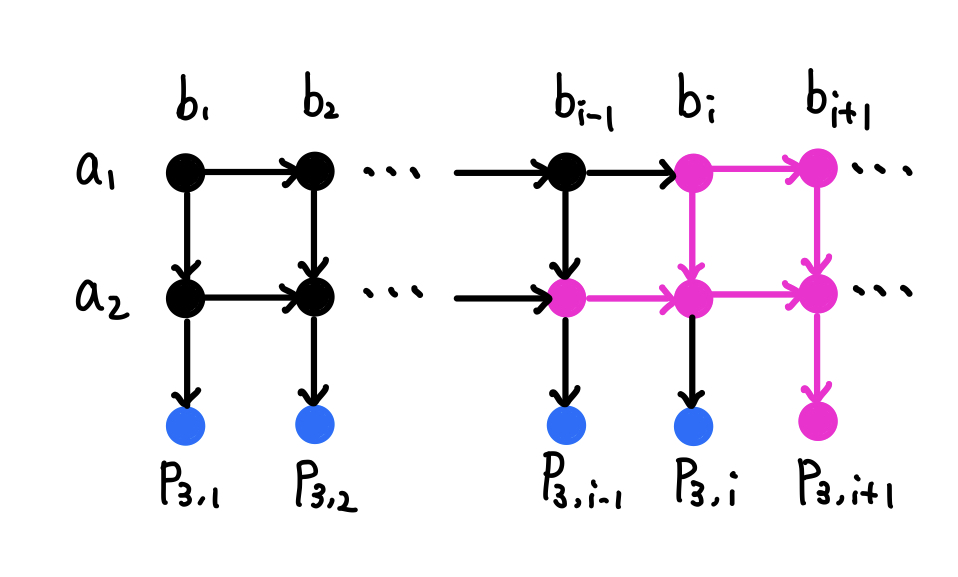
\includegraphics[width=0.6\textwidth]{Fig-stateDiagram2.jpeg}
        \caption{State-transition diagram of a special case}
        \label{ex462}
	\end{figure}\\
It's obvious that $P_{3,1} = P'_{3,1}$. Also, $P_{3,2} = P'_{3,2}$ is very easy to prove.\\
We assume, for any $k\leq i, (i\geq 2)$:
$$P_{3,k} = P'_{3,k}$$
Then, according to the relation formula of vertices given above, we get:
$$\begin{aligned} P_{3,i-1} &= P_{2,i-1}  \cdot  \frac{b_{i-1}} {a_2+b_{i-1}}\\
P_{3,i} &= P_{2,i}  \cdot  \frac{b_{i}} {a_2+b_{i}}\\
P_{3,i+1} &= P_{2,i+1}  \cdot  \frac{b_{i+1}} {a_2+b_{i+1}}\\
P_{2,i} &= P_{2,i-1} \cdot  \frac{a_{2}} {a_{2}+b_{i-1}} + P_{1,i} \cdot  \frac{b_{i}} {a_{1}+b_{i}}\\
P_{2,i+1} &= P_{2,i} \cdot  \frac{a_{2}} {a_{2}+b_{i}} + P_{1,i+1} \cdot  \frac{b_{i+1}} {a_{1}+b_{i+1}}\\
P_{1,i+1} &= P_{1,i} \cdot  \frac{a_1} {a_1+b_{i}}
\end{aligned} $$
The unknown variables in these 6 equations corresponds to the 6 pink vertices in Figure \ref{ex462}. By solving them, we get:
$$\begin{aligned} P_{3,i+1} &= \frac{a_1 a_2M+(a_1+a_2)N}{b_{i-1}b_{i}^2(a_1+b_{i+1})(a_2+b_{i+1})}\\
M &= b_{i+1}(P_{3,i}(b_{i+1}b_{i-1}+b_{i-1}b_{i})-P_{3,i-1}b_{i}b_{i+1})\\
N &= b_{i-1}b_{i}b_{i+1}^2P_{3,i} \end{aligned}$$
It's easy to see $a_1$ and $a_2$ are symmetrical for $P_{3,i+1}$. Also, because $P_{3,i-1} = P'_{3,i-1}$ and $P_{3,i} = P'_{3,i}$. Therefore:
$$P_{3,i+1} = \frac{a_1 a_2M+(a_1+a_2)N}{b_{i-1}b_{i}^2(a_1+b_{i+1})(a_2+b_{i+1})} = \frac{a_2 a_1M'+(a_2+a_1)N'}{b_{i-1}b_{i}^2(a_2+b_{i+1})(a_1+b_{i+1})}=P'_{3,i+1}$$
Then, by mathematical induction, we successfully prove lemma 1.\\\\
{\color{blue}Lemma 2:} If there are two or more than two robots in team A, the probability of A losing the game won't change after switching the order of two arbitrary neighboring robots.\\\\
{\color{blue}Proof Lemma 1:}  The corresponding state-transition diagram is shown in Figure \ref{ex463}.\\
	\begin{figure}[htbp]
	    \centering
        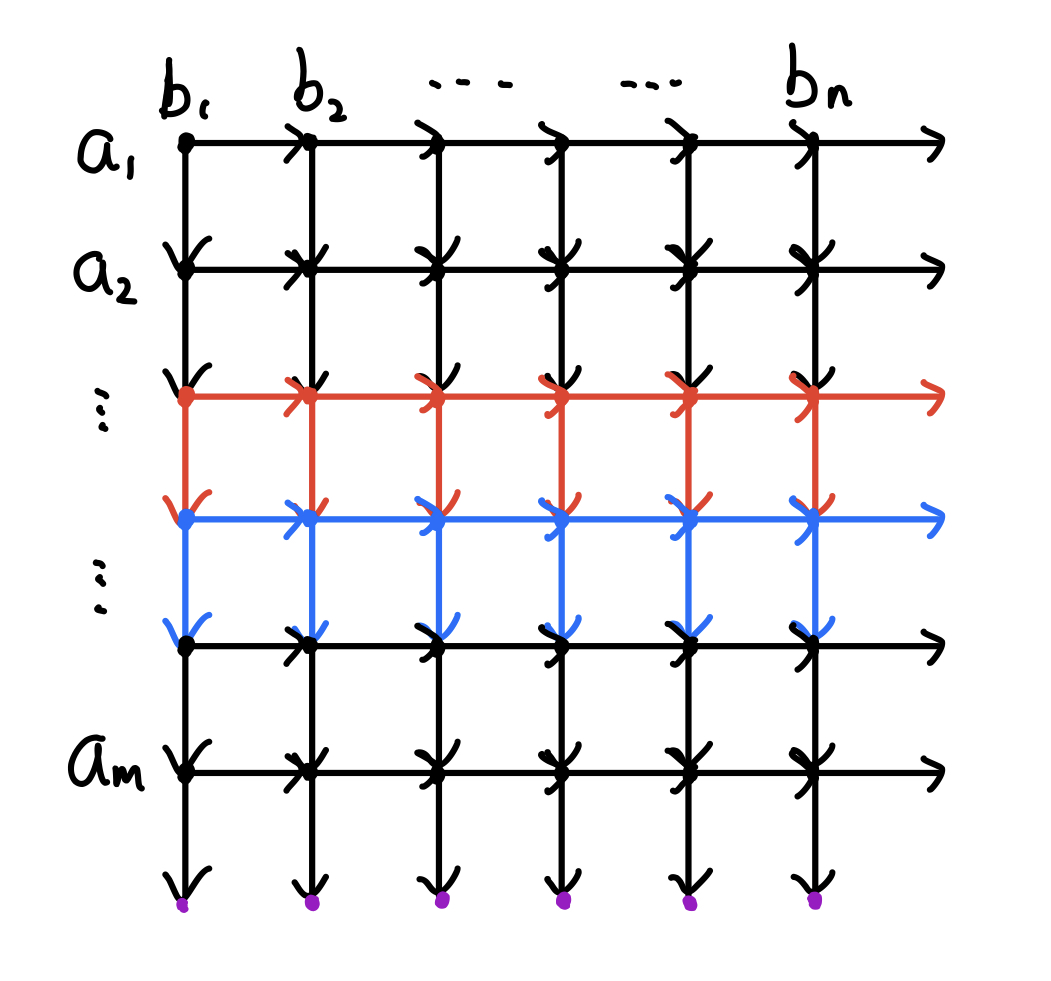
\includegraphics[width=0.5\textwidth]{Fig-stateDiagram3.jpeg}
        \caption{State-transition diagram of general case}
        \label{ex463}
	\end{figure}\\
We zoom in and construct a new diagram shown as Figure \ref{ex464}.\\
	\begin{figure}[htbp]
	    \centering
        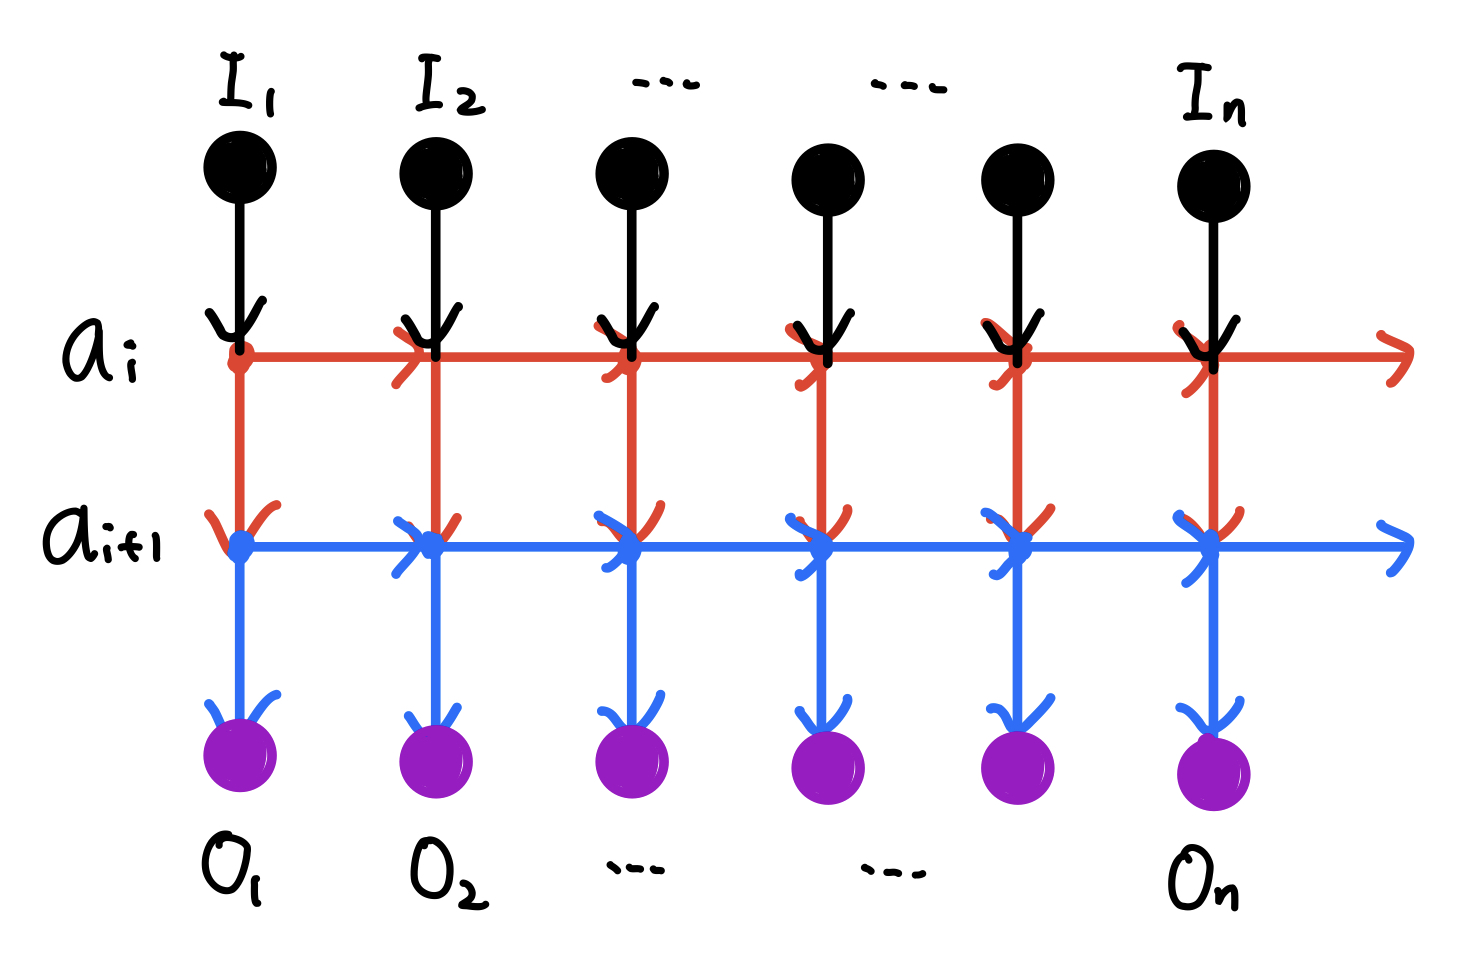
\includegraphics[width=0.5\textwidth]{Fig-stateDiagram4.jpeg}
        \caption{Constructed state-transition diagram}
        \label{ex464}
	\end{figure}\\
$I_k$ is the input corresponding to $P_{i-1,k}$(when $i=1$, then $I_1=1$, $I_k=0$ for $k\in{2,3,\cdots,n}$). $O_k$ is the output. \\
To prove lemma 2, we only have to prove: given inputs, outputs won't change after switching.\\
Suppose $I_0=1$ while other inputs are zero, we get outputs $(O_1^{<1>},O_2^{<1>},\cdots,O_n^{<1>})$. Similarly, suppose $I_j=1$ while other inputs are zero, we get outputs $(O_1^{<j>},O_2^{<j>},\cdots,O_n^{<j>})$. Actually $O_k^{<j>}=0$ when $k<j$. It's shown in Figure \ref{ex465}\\
 	\begin{figure}[htbp]
	    \centering
        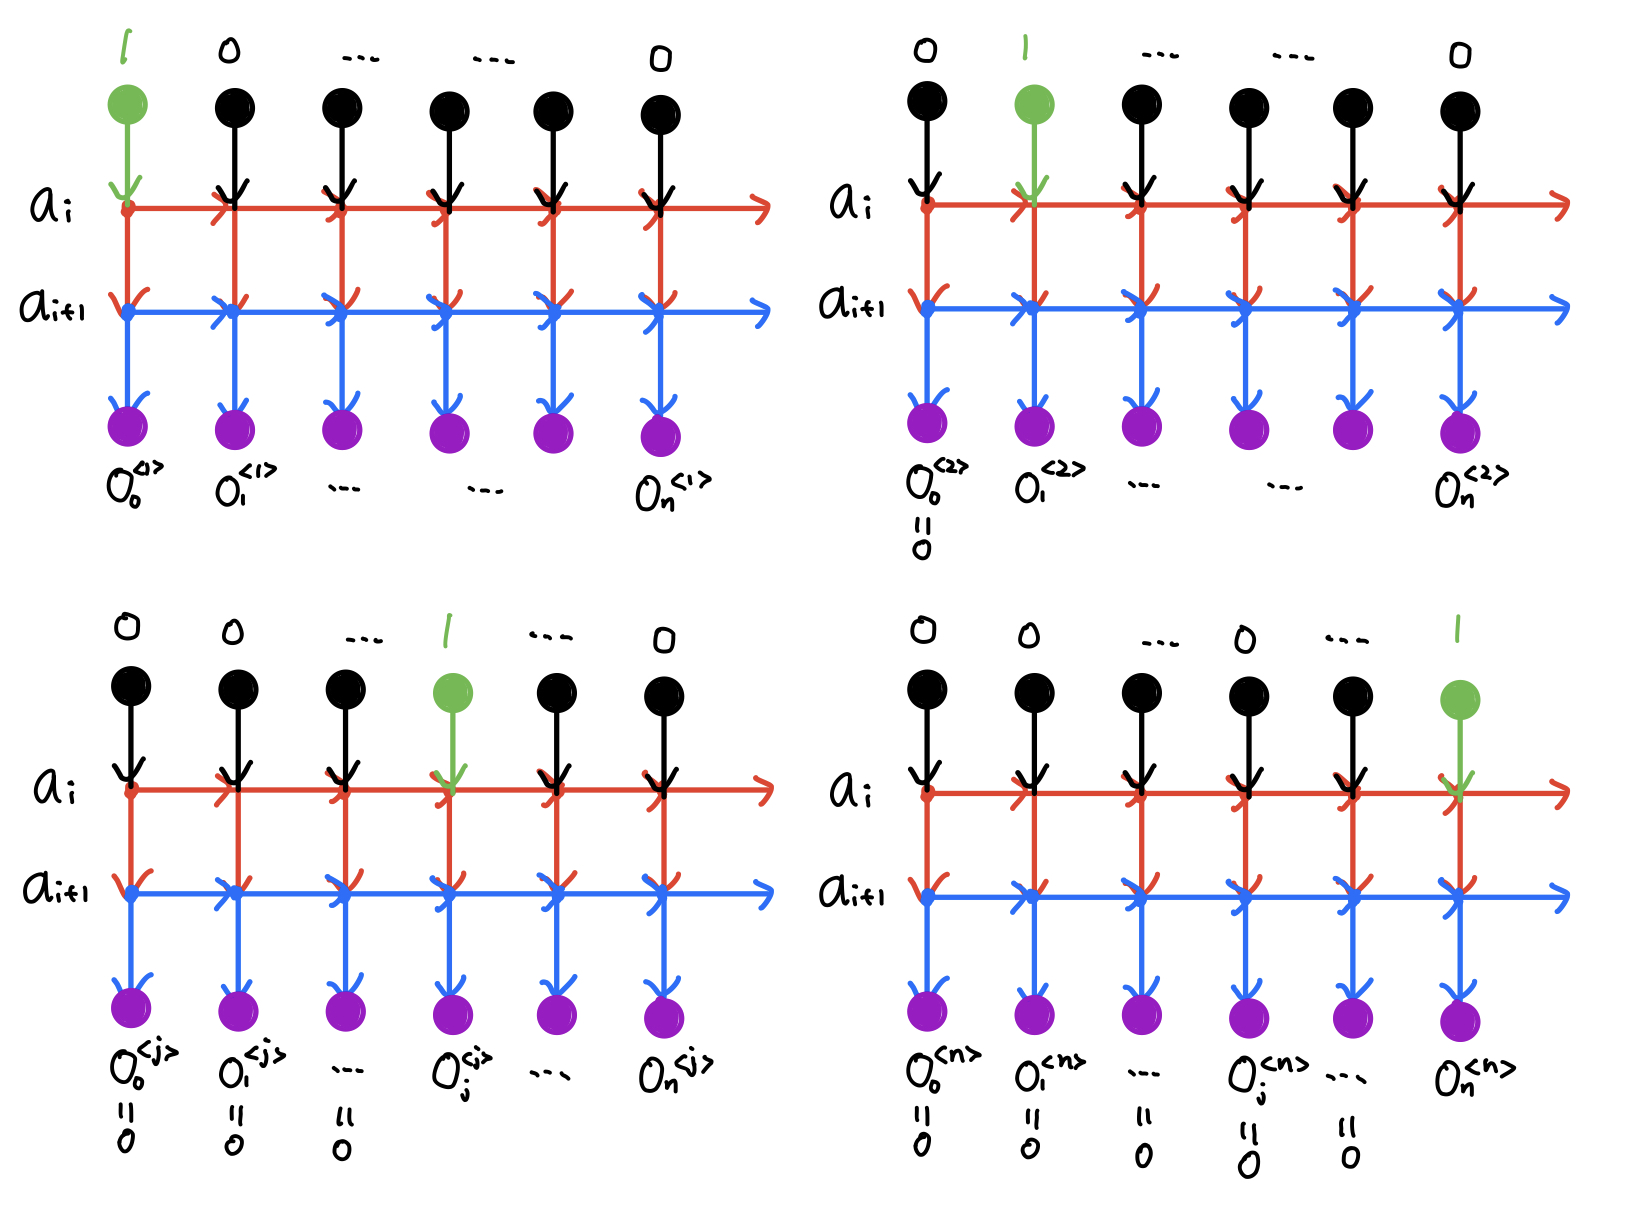
\includegraphics[width=0.8\textwidth]{Fig-stateDiagram5.jpeg}
        \caption{Divided state-transition diagram}
        \label{ex465}
	\end{figure}\\
It's easy to get that: 
$$O_k = \sum_{j=1}^n I_j\cdot O_k^{<j>}$$
According to our lemma 1, $O^{<j>}$ won't change when after switching. Therefore, $O$ won't change after switching. Then we successfully prove lemma 2.\\\\
{\color{blue}Proof Exercise 4.6:} As a truth, given a sequence $(1,2,\cdots,n)$, we can get any permutation of this sequence by constantly switching two neighboring elements.\\
According to Lemma 2, the probability of winning stays unchanged after switching two neighboring robots of team A. It's also true that probability of winning stays unchanged after switching two neighboring robots of team B. \\We can get any sequence of team A and team B after constantly switching. Therefore, the probability of Alice's team winning does not depend on the order in which Alice and Bob send their robots into the arena

%----------------------------END----------------------------






\end{document}

